\documentclass[a4paper,11pt]{article}
\usepackage[utf8]{inputenc}
\usepackage[T1]{fontenc}
\usepackage[french]{babel}
\usepackage{makeidx}
\usepackage{textcomp}
\usepackage{graphicx}
\usepackage{mathtools,amssymb,amsthm}
\usepackage{lmodern}
\usepackage{multirow}
\usepackage{listings}
\usepackage{array}
\usepackage{longtable}
\usepackage{pdfpages}

\title{TER 2019 - Rapport}
\author{Maxime Gonthier - Benjamin Guillot - Laureline Martin}

\begin{document}
\pagenumbering{gobble}\clearpage
\maketitle

\newpage
\tableofcontents

\newpage
\section{Introduction}
	Le projet décrit dans ce rapport est la réalisation d'Algorithmes d'optimisation pour un bureau des temps.\\
	La mission d'un tel bureau est de permettre une décongestion des moyens et infrastructure de mobilité afin d'améliorer la qualité de vie des utilisateurs et de diminuer l'impact environnemental de ces structures. Il s'agira donc d'influer sur les causes de la congestion de mobilités en repensant les horaires d'activités.\\
	Dans notre projet, les horaires d'activités sont celles de l'Université Versailles-Saint-Quentin, et plus précisément de l'UFR des Sciences, basé à Versailles. L'objectif sera ici de minimiser le nombre d'étudiants par bus pour ainsi éviter de fortes congestion. Pour cela, on influera sur les horaires de début de cours pour un emploi du temps journalier. Ainsi en repensant ces horaires, on pourra minimiser la congestion sur la ligne de bus R, allant de la gare transilien Versailles-Chantier à l'UFR.\\
	\\
	Ce rapport a pour objectif de décrire dans un premier temps les données que nous allons utiliser dans notre projet. Ensuite, nous définirons les objectifs à atteindre et les stratégies de résolutions envisagées afin d'atteindre ces objectifs. Nous comparerons ensuite pour ces différentes stratégies les résultats obtenus afin d'identifier la meilleure stratégie.\\
	Afin de faciliter la compréhension de ce rapport, nous allons expliciter les étapes sous la forme d'un exemple simple situé en annexes.
	
	
\section{Les données initiales}
	Cette section fait l'état des données utilisées pour le bon fonctionnement de l'application.\\
	Nous avons pour but de créer une planification pour un emploi du temps, c'est-à-dire un déroulement sur une journée des cours dans une université, ici l'UFR de Versailles.\\
	\\
	L'idée étant de modifier un emploi du temps afin de minimiser la congestion dans les bus dûe aux arrivées d'étudiants au début de leurs cours. Il nous faut donc un emploi du temps de base sur lequel travailler.\\

	Nos données initiales sont :
	\begin{itemize}
		\item Probabilité de lien entre deux cours (un lien est au moins un étudiant en commun entre deux cours)
		\item Le nombre cours
		\item Le nombre de salles 
		\item Le type de chaque cours 
		\item L'heure de début et de fin de journée
		\item Le lapse de temps entre la fin d'un cours et le début du suivant
	\end{itemize}

	La probabilité de lien entre deux cours est définis entre 0 et 1. Les cours sont considérés comme les sommets d'un graphe. Si nous voulons un degré moyen K dans notre graphe, alors on doit mettre une probabilité de lien de K/N avec N le nombre cours.

	Une fois les liens générés, on représente le graphe sous la forme d'une matrice d'adjacence. \\
	Cette représentation nous permet de facilement identifier quels cours ont des étudiants en communs.\\
	\\
	\begin{tabular}{ | c | c | c | c |}
		\hline			
		\       & Cours 1 & Cours 2 & Cours 3\\
		Cours 1 &   0     &    1    &     0  \\
		Cours 2 &   1     &    0    &     0  \\
		Cours 3 &   0     &    0    &     0  \\
		\hline  
	\end{tabular}\\
	Dans cette exemple, nous pouvons voir que le cours 1 et le cours 2 ont au moins un étudiant en commun.\\
	Nous avons besoin de cette information afin de pouvoir fournir une planification réaliste.\\
	\\
	Le nombre de salle sera dans notre graphe le nombre couleur utilisé au maximum pour colorier les sommets.
	Chaque cours est également défini par son type :
	\begin{itemize}
		\item un CM
		\item  un TD
	\end{itemize}
	Ces informations seront utilisées pour connaitre le nombre d'élèves arrivés à chaque cours. En effet, chaque type de cours a un nombre différent d'élèves.\\
	L'heure de début de journée corespond à l'horaire minimale de début d'un cours.
	Le lapse de temps entre deux cours correspond au temps laissé entre deux cours, dans notre cas on fixe cette valeur à 15 minutes.
	Avec les données initiales décrite ci dessus nous pourrons créer un emploi du temps initial.
	
\section{Objectif}
	L'objectif de notre projet est de générer un emploi du temps, c'est-à-dire une planification qui respecte toutes les contraintes et dont la métrique est minimale.
	\subsection{Contraintes}
		\subsubsection{Entre deux cours}
			\begin{enumerate}
				\item Deux cours utilisent la même salle ne doivent pas avoir des horaires qui se chevauchent.
				\item Deux cours qui ont des horaires qui se chevauchent ne doivent pas avoir d'élèves en commun.
				\item Le temps laissé entre deux cours doit être de 15 minutes minimum.
			\end{enumerate}
	
	\subsection{Métriques sur les contraintes}
		Nous évaluons le dépassements du seuil de confort du bus. Dans notre cas d'étude, le seuil de confort est fixé à 50 personnes. Au delà de ce seuil, le score de congestion est incrémenté à chaque arrêt de bus.
		Le nombre d'étudiants dans un bus ne doit pas dépasser la capacité $capacité_{max}$ du bus. Cette capacité maximale est fixée à 60 dans notre cas d'étude. Ainsi s'il y a plus de 60 élèves pour un bus, le surplus d'élèves empruntera le bus précédent l'horaire du bus surchargé.\\
		Pour calculer le nombre d'élèves par bus, on utilise l'emploi du temps des données initiales. Nous pouvons ainsi récupérer pour chaque tranche horaire le nombre d'étudiants censé arriver pour suivre leur cours.\\
		Nous posons l'hypothèse que les élèves arrivent dans le bus précédant leur cours, de ce fait on peut savoir précisément le nombre d'élèves qu'il y aura dans un bus avant un cours.\\
		On prend également en compte le fait que chaque bus comporte une part de non-étudiants, qui ne sera donc pas variable dans notre application. En effet, une modification de la planification ne changera pas leur nombre.\\
		A partir de ces informations, nous pouvons savoir si un bus atteint son seuil de congestion.
		
	\subsection{Objectif}
		La métrique décrite dans le point précédent va nous permettre de donner un score a chaque planification que nous allons réaliser.\\
		En effet, l'objectif étant de réduire la congestion des bus, nous aurons tendance à préférer une planification pour laquelle le score de congestion est faible.\\
		C'est donc dans la modification de la planification que les contraintes vu plus haut interviennent.\\
		Nous allons donc devoir trouver une planification qui minimise la congestion des bus tout en respectant les trois contraintes vu précédemment.
	
\section{Stratégies de résolution}
	\subsection{Planification initiale}
		Dans un premier temps, nous allons créer une planification initiale qui sera utilisée comme point de départ par chaque algorithme. Cette solution va simplement mettre le sommet initial à la première horaire de la journée puis placer les autres sommets en respectant les contraintes et en les mettant le plus tôt possible. Le sommet initial est le sommet de degré entrant nul d'indice le plus faible. Ces sommets sont les cours, représenté dans la matrice d'adjacence vu dans le premier point de ce rapport.\\
		En pseudocode on a :\\
		\begin{lstlisting}
Mettre le sommet de degre entrant nul d indice minimale a l horaire minimale
Pour chaque sommet sauf le premier sommet :
  Mettre l horaire le plus tot respectant les contraintes.
		\end{lstlisting}

	\subsection{Les algorithmes}
		\subsubsection{L'algorithme glouton}
			Cet algorithme est basé sur une heuristique simple : à partir d'une planification initiale, on fait varier les cours un par un sur toutes les horaires possibles respectant les contraintes.\\
			Pour chaque modification on recalcule la congestion des bus. Si la congestion est améliorée, alors on défini cet horaire comme étant le nouvel horaire du cours.\\
			On parcours cependant toutes les horaires possibles afin de choisir celui qui améliore le plus la congestion. Si aucun n'améliore la congestion, le cours est placé à son horaire initial.\\
			Une fois le premier sommet fixé, le sommet suivant est traité et ainsi de suite.\\
			En pseudocode on a :\\
\begin{lstlisting}
Pour chaque sommet :
  Pour chaque horaire :
  	Si la planification a cette horaire respecte les contraintes :
    	Calculer la nouvelle congestion.
    	Si la congestion est meilleur qu'avant le changement,
      	on fixe ce sommet a ce nouvel horaire et on reitere. 
    Sinon, on replace le sommet a son horaire initial 
      et on passe au sommet suivant.
		\end{lstlisting}

		\subsubsection{L'algorithme tabou dur}
			Cet algorithme est basé sur le même principe que pour l'algorithme glouton mais d'une façon différente.\\
			Pour chaque cours, l'heure de début varie tout en respectant les contraintes et une nouvelle valeur pour la congestion est calculée. La meilleure modification pour chaque sommet est gardée en mémoire.\\
			Après avoir effectué cette recherche sur tout les cours de la planification, le sommet ayant la meilleure amélioration de congestion est modifié.\\
			Ce procédé est ensuite répété mais en interdisant l'optimisation d'un cours dont l'horaire a déjà été modifiée.\\
			En pseudocode on a :\\
\begin{lstlisting}
Pour chaque sommet :
  Pour chaque horaire :
  	Si la planification a cette horaire respecte les contraintes :
    	Calculer la nouvelle congestion.
    	Si la congestion est meilleur qu'avant le changement,
      	on la conserve.
  On selectionne la meilleure congestion. 
  On modifie l'horaire du sommet associe a cette congestion a l'horaire donnant cette congestion
		\end{lstlisting}

		\subsubsection{L'algorithme tabou roulette}
			Cet algorithme ressemble à l'algorithme tabou dur, à ceci près qu'il laisse une part de hasard dans le choix de la modification à apporter dans la planification.\\
			En effet, cet algorithme traite toutes les horaires respectants les contraintes pour tous les cours. La congestion est ensuite calculée pour chaque horaire.\\
			Ensuite, parmi toute les solutions de tous les sommets, une seule est choisie aléatoirement. Cependant, plus une solution améliore la congestion, plus elle aura de chance d'être sélectionnée. C'est le même fonctionemment qu'une roulette dont les sous parties ne sont pas de tailles égales.\\
			L'opération est ensuite réitérée tout en interdisant l'optimisation d'un cours déjà modifié, comme pour l'algorithme précédent.\\
			En pseudocode on a :\\
\begin{lstlisting}
Pour chaque sommet :
  Pour chaque horaire :
  	Si la planification a cette horaire respecte les contraintes :
    	Calculer la nouvelle congestion.
    	Si la congestion est meilleur qu'avant le changement,
      	on la conserve.
  Chaque valeur de congestion est associe a une valeur proportionelle au taux de modification par rapport a la planification initiale
  On choisit un nombre au hasard. Le sommet associe a la congestion choisis change son horaire a l horaire donnant cette congestion.
  \end{lstlisting}
	
	\subsection{Données utilisées}
		Voir l'exemple en annexe pour plus de clarté.

		\subsubsection{Le nombre de personnes par bus}
			Dans notre cas d'étude, nous considérons que tous les étudiants montent au premier arrêt (gare des chantiers) et descendent au terminus (l'université).\\
			Nous allons aussi créer le nombre de montées et de descentes à chaque arrêt.
 			Pour obtenir les données des arrêts intermédiaires nous choisirons une valeur aléatoire, choisie dans un intervalle différent en fonction de l'heure. L'objectif est de représenter la congestion forte des heures de pointes de manière un peu plus précise : \\
 			\begin{tabular}{ | c | c | c | c | c | c | c | c | c | c |}
 				\hline			
   				Horaire & 7-8h & 8-9h & 9-10h & 10-11h & 11-12h & 12-13h & 13-14h & 14-15h & 15-16h\\
   				Montées & [5:15] & [5:15] & [3:10] & [2:8] & [1:5] & [1:5] & [1:5] & [2:8] & [3:10]\\
   				Descentes & [0:5] & [0:5] & [1:6] & [1:6] & [1:5] & [1:5] & [0:5] & [0:5] & [1:5]\\
 				\hline  
 			\end{tabular}\\

	\subsection{L'emploi du temps}
		L'emploi du temps est un graphe dont les sommets sont des cours et les liens des étudiants en communs.
		Pour plus de clarté nous considérons ici que chaque professeur est disponible sur toute la durée de la journée.\\
		Les sommets du graphe sont également coloriés, chaque couleur représentant une salle.
		\begin{enumerate}
			\item On crée un graphe non orienté en numérotant les sommets de 1 jusqu'au nombre de cours.
			\item On relie les sommets entre eux lorsque qu'il y a une contrainte (étudiants en commun). Pour cela on crée une matrice d'adjacence avec un degré moyen choisit arbitrairement. Pour $N$ sommets et $K$ le degré moyen, la probabilité qu'il y ai une arête à insérer dans chaque case est $K/N$.
			\item Les arêtes s'oriente, désormais des arcs, du sommet d'indice le plus faible au plus fort
			\item Il y a obligatoirement un ou plusieurs sommets de degré entrant nul, ces sommets de notre DAG seront des points de départs possible pour notre planification.
			\item Le graphe est colorié, chaque couleur représente une salle.		
			\item L'emploi du temps est agencé en respectant le fait que deux couleurs et deux sommets reliés par un arc ne peuvent pas être sur la même plage horaire. Par défaut le sommet duquel nous partirons est le sommet de degré entrant nul d'indice le plus faible.
		\end{enumerate}
		Chaque cours possède un nombre d'étudiants choisit aléatoirement entre 16 et 32 pour un TD et entre 16 et 100 pour un cours magistral. les TDs représentent trois quart des cours.\\
		\\	
		Cependant comme nous avons dû les générer faute de données concrètes, nous inclurons également dans cette section l'ensemble des variables utilisées pour les générer.

	\subsection{Les variables}
		Les noms des variables sont simplifiés par rapport à leur nom réel dans l'application afin de les rendre plus explicite pour le lecteur.
		\begin{itemize}
			\item \textit{probabilité de lien} : la probabilité qu'il y ai un lien entre 2 cours. Un lien entre 2 cours signifie qu'ils ont au moins un étudiant en commun, ils ne peuvent donc pas avoir lieu en même temps.
			\item \textit{nombre de cours} : le nombre de cours que nous allons représenter lors du déroulement de l'application. C'est le nombre de cours que nous allons devoir modifier pour la planification.
			\item  \textit{le nombre de salles} : le nombre de salles disponibles pour les cours.
			\item \textit{heure maximum} : l'heure limite à laquelle on peut placer un cours. Dans notre cas d'étude, nous représentons le temps par tranche de 15 minutes. Il va de 7h30 à 16h, on à donc 34 quart d'heure.
		\end{itemize}

\section{Présentation et analyse des résultats}
	Nous allons tester nos algorithmes en choisissant différentes valeurs de degré moyen. Nous fixons le nombre de cours à 40. Par exemple pour un degré moyen de 3 on calcule la probabilité de lien entre deux cours à utiliser : 40/3 = 0.075. Le nombre de salles est fixé à 30. On itère les algorithmes tabou sur 10 itérations. Les valeurs affichées sont le nombre de bus totalement congestionés.\\
	
	Ce tableau représente le nombre de bus congestionés par méthode. Le degré moyen du graphe est 1 (0.025 probabilité de lien entre deux cours).\\ 
	\begin{tabular}{|c|c|c|c|c|}
  		\hline
  		Tirage numéro & Initiale & Algo glouton & Algo tabou dur & Algo tabou roulette\\
  		\hline
  		1 & 9 & 9 & 9 & 9\\
  		\hline
  		2 & 10 & 10 & 10 & 10\\
  		\hline
  		3 & 11 & 8 & 8 & 8\\
  		\hline
  		4 & 10 & 10 & 10 & 10\\
  		\hline
  		5 & 10 & 10 & 10 & 10\\
  		\hline
  		6 & 10 & 8 & 9 & 8\\
  		\hline
  		7 & 10 & 10 & 10 & 10\\
  		\hline
  		8 & 12 & 12 & 12 & 12\\
  		\hline
  		9 & 10 & 10 & 10 & 10\\
  		\hline
  		10 & 16 & 9 & 10 & 11\\
  		\hline
  		11 & 9 & 9 & 9 & 9\\
  		\hline
  		12 & 10 & 10 & 10 & 10\\
  		\hline
  		13 & 11 & 11 & 11 & 11\\
  		\hline
  		14 & 10 & 10 & 10 & 10\\
  		\hline
  		15 & 10 & 10 & 10 & 10\\
  		\hline
  		Moyenne & x & x & x & x\\
  		\hline
	\end{tabular}

	Ce tableau représente le nombre de bus congestionés par méthode. Le degré moyen du graphe est 5 (0.125 probabilité de lien entre deux cours).\\ 
	\begin{tabular}{|c|c|c|c|c|}
  		\hline
  		Tirage numéro & Initiale & Algo glouton & Algo tabou dur & Algo tabou roulette\\
  		\hline
  		1 & 13 & 6 & 11 & 7\\
  		\hline
  		2 & 11 & 9 & 7 & 8\\
  		\hline
  		3 & 12 & 7 & 7 & 7\\
  		\hline
  		4 & 10 & 9 & 8 & 8\\
  		\hline
  		5 & 14 & 9 & 10 & 8\\
  		\hline
  		6 & 12 & 7 & 7 & 8\\
  		\hline
  		7 & 13 & 8 & 9 & 6\\
  		\hline
  		8 & 12 & 10 & 12 & 10\\
  		\hline
  		9 & 11 & 8 & 9 & 8\\
  		\hline
  		10 & 12 & 7 & 7 & 7\\
  		\hline
  		11 & 10 & 9 & 9 & 8\\
  		\hline
  		12 & 11 & 10 & 10 & 10\\
  		\hline
  		13 & 16 & 7 & 8 & 10\\
  		\hline
  		14 & 10 & 7 & 6 & 6\\
  		\hline
  		15 & 10 & 7 & 7 & 8\\
  		\hline
  		Moyenne & X & X & X & X\\
  		\hline
	\end{tabular}

	Ce tableau représente le nombre de bus congestionés par méthode. Le degré moyen du graphe est 7 (0.175 probabilité de lien entre deux cours).\\ 
	\begin{tabular}{|c|c|c|c|c|}
  		\hline
  		Tirage numéro & Initiale & Algo glouton & Algo tabou dur & Algo tabou roulette\\
  		\hline
  		1 & 8 & 6 & 6 & 5\\
  		\hline
  		2 & 10 & 9 & 9 & 9\\
  		\hline
  		3 & 11 & 7 & 8 & 9\\
  		\hline
  		4 & 10 & 10 & 7 & 9\\
  		\hline
  		5 & 13 & 8 & 8 & 11\\
  		\hline
  		6 & 10 & 8 & 8 & 8\\
  		\hline
  		7 & 9 & 8 & 8 & 8\\
  		\hline
  		8 & 12 & 8 & 9 & 9\\
  		\hline
  		9 & 13 & 4 & 5 & 5\\
  		\hline
  		10 & 11 & 7 & 7 & 8\\
  		\hline
  		11 & 9 & 8 & 8 & 9\\
  		\hline
  		12 & 12 & 7 & 8 & 7\\
  		\hline
  		13 & 10 & 9 & 9 & 9\\
  		\hline
  		14 & 13 & 8 & 10 & 8\\
  		\hline
  		15 & 9 & 8 & 7 & 8\\
  		\hline
  		Moyenne & X & X & X & X\\
  		\hline
	\end{tabular}

	Ce tableau représente le nombre de bus congestionés par méthode. Le degré moyen du graphe est 10 (0.25 probabilité de lien entre deux cours).\\ 
	\begin{tabular}{|c|c|c|c|c|}
  		\hline
  		Tirage numéro & Initiale & Algo glouton & Algo tabou dur & Algo tabou roulette\\
  		\hline
  		1 & 12 & 8 & 7 & 7\\
  		\hline
  		2 & 13& 8& 8&8\\
  		\hline
  		3 & 11 & 7 & 6 & 8\\
  		\hline
  		4 & 13 & 8 & 10 & 9\\
  		\hline
  		5 & 12 & 8 & 9 & 7\\
  		\hline
  		6 & 10 & 8 & 6 & 6\\
  		\hline
  		7 & 13 & 7 & 8 & 8\\
  		\hline
  		8 & 11 & 10 & 9 & 10\\
  		\hline
  		9 & 15 & 8 & 8 & 9\\
  		\hline
  		10 & 11 & 8 & 9 & 7\\
  		\hline
  		11 & 10 & 6 & 9 & 6\\
  		\hline
  		12 & 12 & 9 & 6 & 6\\
  		\hline
  		13 & 8 & 6 & 6 & 7\\
  		\hline
  		14 & 9 & 7 & 7 & 7\\
  		\hline
  		15 & 9 & 8 & 9 & 7\\
  		\hline
  		Moyenne & X & X & X & X\\
  		\hline
	\end{tabular}

	Comparer les algos, comparer en fct des données en entrées
	Moyenne de l'algo tabou roulette sur la meme horaire.
	
\section{Conclusion}
	\subsection{Pistes de reflexion abandonnées}
		Lors de nos recherches préliminaires, nous avions pensé représenter chaque éléments (cours, étudiants, professeurs, salles) par des classes. Ainsi, un langage de programmation orienté objet nous semblait tout indiqué. Mais nous savions également que nous allions avoir besoin de fonctions procédurales (les algorithmes par exemple). Donc, nous avons opté pour l'utilisation du langage C++ qui est un langage hybride\\
		Au cours de nos recherches, nous nous sommes rendu compte que nous pouvions modéliser notre problème en utilisant simplement des matrices, nous avons donc abandonnée l'idée de représenter les éléments du projets par des objets.\\
		Cependant, comme nous avions déjà commencé à programmer une partie du projet, nous avons décidé de garder le C++ comme langage de programmation, sont aspect hybride entre le procédural et l'orienté objet nous permettant de continuer a l'utiliser.
	
	\subsection{Conclusion sur les objectifs initiaux}
		Le problème d'optimisation pour un bureau des temps n'a pas de solution simple. Nous avons eu recourt à différentes heuristique afin de pouvoir fournir des planifications viables.\\
		Ce problème est donc assez coûteux en temps en fonction de l'heuristique choisie. De plus, nous ne pouvons pas affirmer à 100\% que les planifications fournies soient les meilleures. Cependant, nous pouvons essayer de s'en approcher.

	\subsection{Ouverture}
		Nous avons quelques pistes de réflexions qui pourraient améliorer l'efficacité de notre application.\\
		Il serait possible par exemple de donner aux algorithmes la possibilité d'inverser les arcs de la matrice d'adjacence des cours. Ainsi on ne serait pas limité à l'ordre établi lors de la planification initiale (a ré-expliquer mieux).\\
		Il serait également possible d'essayer d'utiliser d'autres heuristiques que celles que nous avons choisi. comme un recuit simulé par exemple (à expliquer), ou alors changer la variable de décision (à expliquer) de l'algorithme glouton.


\newpage
\section{Annexes}
	\subsection{Exemple d'utilisation}
		\subsubsection{Représentation des montées et descentes du bus}
			Nous considérons que tous les étudiants montent au premier arrêt (gare des chantiers) et descendent au terminus (l'université). On ajoute aussi à chaque arrêt les montées et descentes des non étudiants. Dans notre exemple nous avons : \\
			\\
			\begin{tabular}{ | c | c | c | c | c | c |}
 				\hline			
   				Numéro de l'arrêt	& 1 	& 2 	& 3 	& 4 	& 5\\
   				montées				& 50 	& 15 	& 10 	& 2 	& 0\\
   				Descentes			& 0 	& 5 	& 10 	& 8 	& 54\\
 				\hline  
 			\end{tabular}\\
 			Pour obtenir les données des arrêts intermédiaires de montées et descentes nous choisirons une valeur aléatoire, choisis dans un intervalle différent en fonction de l'heure, l'objectif est de représenter la congestion forte des heures de pointes de manière un peu plus précise : \\
 			\begin{tabular}{ | c | c | c | c | c | c | c | c | c | c |}
 				\hline			
   				Horaire & 7-8h & 8-9h & 9-10h & 10-11h & 11-12h & 12-13h & 13-14h & 14-15h & 15-16h\\
   				Montées & [5:15] & [5:15] & [3:10] & [2:8] & [1:5] & [1:5] & [1:5] & [2:8] & [3:10]\\
   				Descentes & [0:5] & [0:5] & [1:6] & [1:6] & [1:5] & [1:5] & [0:5] & [0:5] & [1:5]\\
 				\hline  
 			\end{tabular}\\

		\subsubsection{L'emploi du temps}
			Voici un exemple de création de la planification initiale : 
			\begin{enumerate}
				\item On créer un graphe non orienté en numérotant les sommets de 1 à 10.
				\centerline{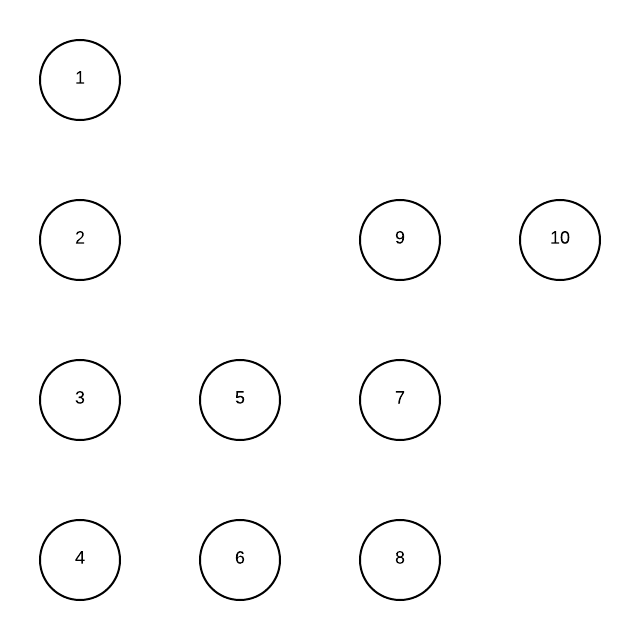
\includegraphics[scale=0.8]{Captures/exemple1.png}}
				\item On relie les sommets entre eux lorsque qu'il y a une contrainte (même étudiant sur des horaires qui se chevauchent). Pour cela on créé une matrice d'adjacence avec un degré moyen choisis arbitrairement. Pour N sommets et K le degré moyen, la probabilité qu'ily ai une arête à insérer dans chaque case est K/N.
				\item On oriente les arêtes désormais des arcs du plus faible au plus fort
				\centerline{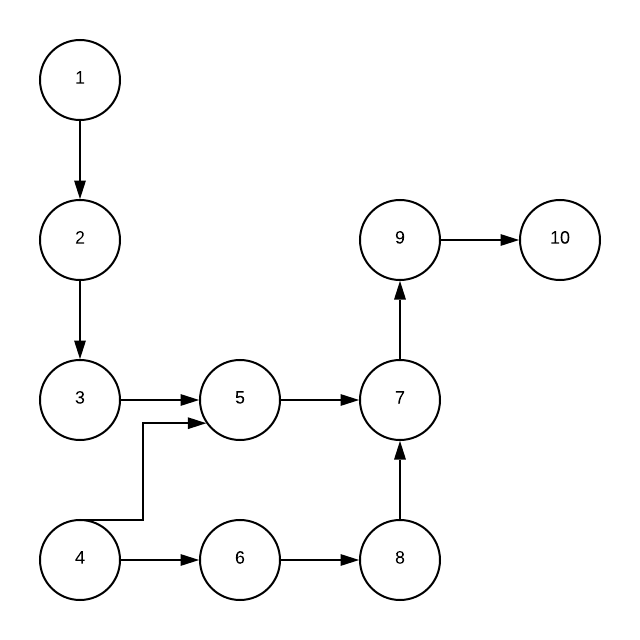
\includegraphics[scale=0.8]{Captures/exemple2.png}}
				\item On remarque dans notre exemple qu'il y a deux sommets de degré entrant nul, ces deux sommets de notre DAG seront des points de départs possible pour notre planification.
				\item On colorie le graphe, chaque couleur représente une salle.\\
				\centerline{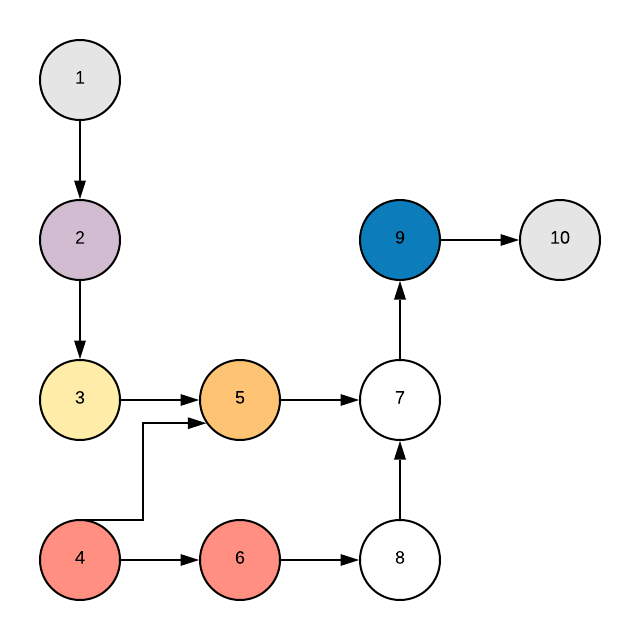
\includegraphics[scale=0.8]{Captures/exemple3.png}}
				\item Nous agencons l'emploi du temps en respectant le fait que deux couleurs et deux sommets reliés par un arc ne peuvent pas être sur la même plage horaire. Par défaut le sommet duquel nous partirons est le sommet de degré entrant nul le plus faible, ici le numéro 1. C'est la planification initiale :
				\\
				\centerline{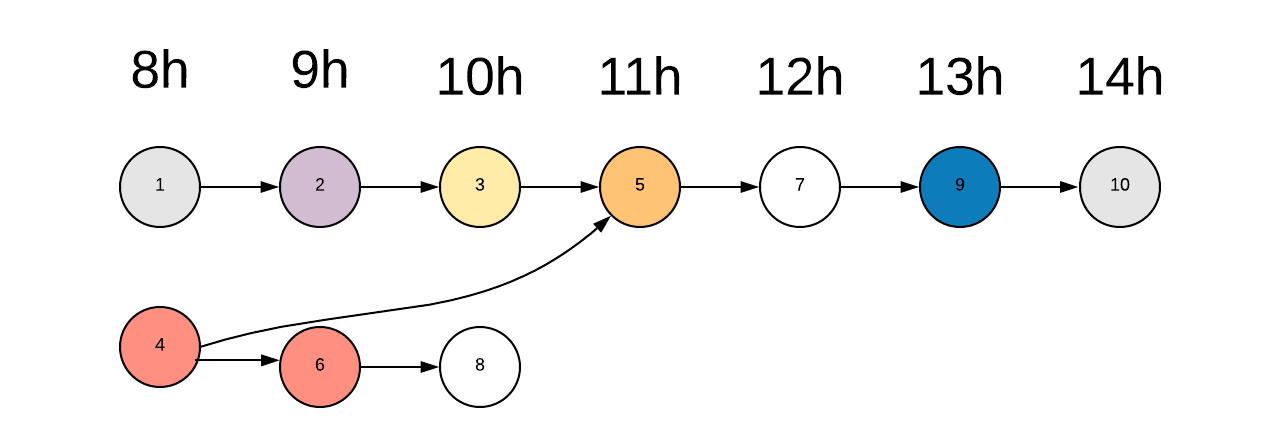
\includegraphics[scale=0.8]{Captures/exemple4.png}}
			\end{enumerate}
			Chaque cours possède un nombre d'étudiants choisis aléatoirement entre 16 et 32 pour un TD et entre 16 et 100 pour un cours magistral. les TDs représentent trois quart des cours. Ainsi dans notre exemple nous avons : \\
			\\
			\begin{tabular}{ | c | c | c | c | c | c | c | c | c | c | c |}
 				\hline			
   				Numéro du sommet & 1 & 2 & 3 & 4 & 5 & 6 & 7 & 8 & 9 & 10\\
   				Type de cour & TD & CM & CM & TD & TD & TD & TD & TD & TD & CM \\
   				Nombre d'élèves & 16 & 70 & 60 & 30 & 25 & 20 & 16 & 30 & 14 & 50\\
 				\hline  
 			\end{tabular}\\

		\subsubsection{Calcul de la congestion}
			A l'aide du tableau ci dessus nous allons pouvoir déterminer à chaque horaire le nombre d'étudiants arrivé au terminus et donc en conclure à l'aide du tableau des montées et des descentes le nombre de personnes à chaque arrêt. 
			On considère que les etudiants prennent le bus arrivant 15 min avant leurs premier cour de la journée.
			Dans notre exemple nous avons pour  8h le cours 1 et 4, ce qui représente 46 élèves. Ainsi le bus de arrivant a 7h45 ressemble à cela :  \\
			\begin{tabular}{ | c | c | c | c | c | c | c |}
 				\hline			
   				Numéro de l'arrêt & 1 & 2 & 3 & 4 & 5\\
   				Différence montées/descentes & 10 & 7 & 10 & 11 & 0\\
   				Nombre de personnes dans le bus & 56 & 53 & 60 & 56 & 57\\
 				\hline  
 			\end{tabular}\\
 			Ce tableau sera générés pour chaque bus. On mesurera dans chaque cas le dépassement à chaque arrêt en mettant un 1 si il y a dépassements, un 0 sinon.
 			Sachant que la limite de confort est de 50 dans le bus que nous étudions, ce bus nous donne une valeur de congestion de 5.\\
 			A partir de la on applique l'algorithme glouton et les deux algorithmes génétiques pour essayer d'améliorer notre fonction objectif.
 			Décrivons ces algos.

	\subsection{Explication de la programmation}
		\subsubsection{Algorithme glouton}
\begin{lstlisting}
//N est le nombre de cours.
for (int i = 0; i < N; i++)
{
	//Horaires_glouton est un tableau contenant la planification 
	//initiale. Chaque case representant l'horaire d'un sommet.
	//Meilleure solution et meilleure congestion representent 
	//respectivement la meilleure horaire pour le sommet i et 
	//la congestion associee a cette horaire.
	//Meilleure horaire signifie horaire qui minimise au plus la 
	//congestion. Avant la boucle on les initialises a l'heure 
	//deja attribue au sommet i.
	sommet_modifie = i;
	meilleure_solution = Horaires_glouton[sommet_modifie];
	meilleure_congestion = calcul_congestion_totale(
		Horaires_glouton,Nb_eleves,
		heure_max,N,TO);
	//Le while test tous les horaires possibles pour le sommet i.
	while(j < heure_max - 1)
	{
		Horaires_glouton[sommet_modifie] = j;
		//Si l'horaire j est valide
		if (test_solution_valide(Horaires_glouton, N, couleur, 
			Type, TO) == true)
		{
			temp = calcul_congestion_totale(Horaires_glouton,
				Nb_eleves,heure_max,N,TO);
			//Si la congestion a l'horaire j est meilleure 
			//que la meilleure congestion du sommet i, 
			//alors on remplace la meilleure congestion et
			//la meilleure horaire par j.
			if(temp < meilleure_congestion)
			{
				meilleure_solution = 
					Horaires_glouton[sommet_modifie];
				meilleure_congestion = temp;
			}
		}
		j++;
	}
	//j commence a 2 car 2 correspond a 8h du matin.
	j = 2;
	Horaires_glouton[sommet_modifie] = meilleure_solution;
}
\end{lstlisting}
		\subsection{Algorithme tabou roulette}
			Nous ne décrivons pas l'algorithme tabou dur car il est quasiment identique. La différence est explicité ci dessous.
\begin{lstlisting}
//Horaires_tabou_roulette est un tableau contenant la planification 
//initiale. Chaque case representant l horaire d un sommet.
int *Horaires_tabou_roulette = (int*)malloc(N*sizeof(int*));

//Tableau qui servira a verifier si un sommet a deja ete modifie 
//et ainsi l interdire
int *Sommets_interdits = (int*)malloc(Nb_iterations*sizeof(int*));

//Tableau contenant la meilleure horaire pour un sommet donne
int *Meilleure_solution = (int*)malloc(N*sizeof(int*));

//Tableau contenant la meilleure solution pour un sommet donne
	int *Meilleure_congestion = (int*)malloc(N*sizeof(int*));

//Tableau contenant les probabilite qu'un sommet sois choisis
//par la roulette
int *Valeurs_roulette = (int*)malloc(N*sizeof(int*));
	
//La boucle k permet d'iterer l'algo plusieurs fois
for(int k = 0; k < Nb_iterations; k++){
	//On initialise la congestion initiale 
	congestion_initiale = calcul_congestion_totale
		(Horaires_tabou_roulette,Nb_eleves,heure_max,N,TO);
	//La boucle i parcoure l'ensemble des sommets
	for(int i = 0; i < N; i++){
		//On cherche a savoir si le sommet courant est un sommet 
		//deja modifie, si oui on ne le regarde pas
		for(int l = 0; l < k+1; l++){
			if(i == Sommets_interdits[l]) {i++; l = 0;}
		}
		//Initialisation des meilleures solution pour le sommet i
		Meilleure_solution[i] = Horaires_tabou_roulette[i];
		Meilleure_congestion[i] = calcul_congestion_totale
			(Horaires_tabou_roulette,Nb_eleves,heure_max,N,TO);
		horaire_initiale = Horaires_tabou_roulette[i];

		//La boucle j parcours l'ensemble des horaires possibles
		while(j < heure_max - 1){
			Horaires_tabou_roulette[i] = j;
			//On verifie que l'horaire est bien valide
			if (test_solution_valide(Horaires_tabou_roulette, 
				N, couleur, Type, TO) == true){
				temp = calcul_congestion_totale(Horaires_tabou_roulette,
					Nb_eleves,heure_max,N,TO);
				//Si la congestion de cette horaire est meilleure, 
				//on met a jour le meilleur horaire et la meilleur 
				//congestion du sommet i
				if(temp < Meilleure_congestion[i]){
					Meilleure_congestion[i] = temp;
					Meilleure_solution[i] = j;
				}
			}
			j++;
		}
		//j commence a 2 car 2 correspond a 8h du matin 
		j = 2;
		//On remet l'horaire du sommet i a son horaire de base 
		//car on sait pas encore quel sommet sera modifie a 
		//cette iteration de l'algo tabou
		Horaires_tabou_roulette[i] = horaire_initiale;
		//On remplit le tableau des proba de cette maniere :
		//On marque la valeurs de modification par rapport a 
		//la congestion initiale. Ainsi si on a 10 de congestion 
		//initiale et 8 en congestion pour le sommet i,
		//Alors on marque 2 dans le tableau. Pour le sommet suivant si 
		//il modifie de 3 on marque 5. 
		//Ainsi ca donne un tableau comme cela : 
		//2 4 8 15 16 17 17.
		if(Meilleure_congestion[i] < congestion_initiale){ 
			Valeurs_roulette[i] = 
				congestion_initiale - Meilleure_congestion[i]; }
		else { Valeurs_roulette[i] = 0; }
	}
	for (int p = 1; p < N; p++) { 
		if (Valeurs_roulette[p] == 0) { 
			Valeurs_roulette[p] = Valeurs_roulette[p-1];} 
		else { Valeurs_roulette[p] += Valeurs_roulette[p-1]; }
	}
		
	if (Valeurs_roulette[N-1] > 0) {
		choix_roulette = rand()%Valeurs_roulette[N-1];
	}
	else { choix_roulette = 0; }

	//On prend au hasard une valeur et on regarde ou elle tombe 
	//dans le tableau, ainsi plus on modifie la congestion, 
	//plus on a de chance d'etre choisi.
	if ((choix_roulette > 0) && (choix_roulette <= Valeurs_roulette[0]))
	{
		Horaires_tabou_roulette[0] = Meilleure_solution[0];
		Sommets_interdits[k] = 0;
	}
	else{
		for (int m = 1; m < N; m++){
			if ((choix_roulette >= Valeurs_roulette[m-1]) 
				&& (choix_roulette <= Valeurs_roulette[m])){
				//Mise a jour de la planification 
				//et des sommets interdits
				Horaires_tabou_roulette[m] = Meilleure_solution[m];
				Sommets_interdits[k] = m;
				m = N;
			}
		}
	}
}
\end{lstlisting}
		\subsubsection{Planification initiale}
\begin{lstlisting}
//N le nombre de cours.
for(int i = 1; i < N; i++){
	//On va regarder tous les liens de i vers k pour tout i et tout k. 
	//Si il y a un lien, le cours i est place avant le cours k. 
	//C'est le sens des arcs qui veut cela.
 for(int k = 0; k < N; k++){
 //Si il y a un lien entre le cours i et le cours k
  if(T[i][k] == 1){
   if(TYPE[i] == 0){//si le cours est un td
    for(int j = 0; j <= 36; j++){
	//Si la solution est valide a l'horaire k + 
	//la duree du cours + une constante j incremente
	//pour tester toutes les possibilites d'horaire.
	 if(test_coloration(Horaires, couleur, N, TYPE, 
		Horaires[k] + 13 + j, i) == true){
		 if(test_lien(Horaires, N, T, Horaires[k]
			+ 13 + j, i, TYPE) == true){
		//On met l'horaire de i avant celle de k.
			Horaires[i] = Horaires[k] + 13 + j;
			break;
		   }
	   }
	 }
    }
	else //si le cours est un cm, le code est le meme.
	{
		for(int j = 0; j <= 36; j++)
		{
			if(test_coloration(Horaires, couleur, N, TYPE, 
				Horaires[k] + 7 + j,i) == true)
			{
			  if(test_lien(Horaires, N, T, Horaires[k] + 7 
				+ j, i, TYPE) == true)
			  {
				Horaires[i] = Horaires[k] + 7 + j;
				break;
			  }
		    }
		  }
	  }
}
//Si il n'y a aucun lien vers le sommet k.
else {
 if(testConnnexe(T, N, i) == true){
  if(TYPE[k] == 0)//si le cours est un td
  {
	for(int j = 0; j <= 36; j++)
	{
	  if(test_coloration(Horaires, couleur, N, TYPE, 
		Horaires[k] + 13  + j, i) == true)
	  {
		if(test_lien(Horaires, N, T, Horaires[k] + 
			13 + j, i, TYPE) == true)
		{
			Horaires[i] = Horaires[k] + 13 + j;
			break;
		}
	}
   }
  }
  else //si le cours est un cm.
  {
	for(int j = 0; j <= 36; j++)
    {
		if(test_coloration(Horaires, couleur, N, TYPE, 
			Horaires[k] + 7 + j,i) == true)
		{
			if(test_lien(Horaires, N, T, Horaires[k] + 
				7 + j, i, TYPE) == true)
			{
				Horaires[i] = Horaires[k] + 7 + j;
			    break;
			}
		}
	}
   }
  }
  }	
 }
}
\end{lstlisting}

\end{document}
